% Figure -- per-layer CKNNA alignment + Platonic off-diagonal. \input{} from Ch6.
\begin{figure}[tbp]
\centering
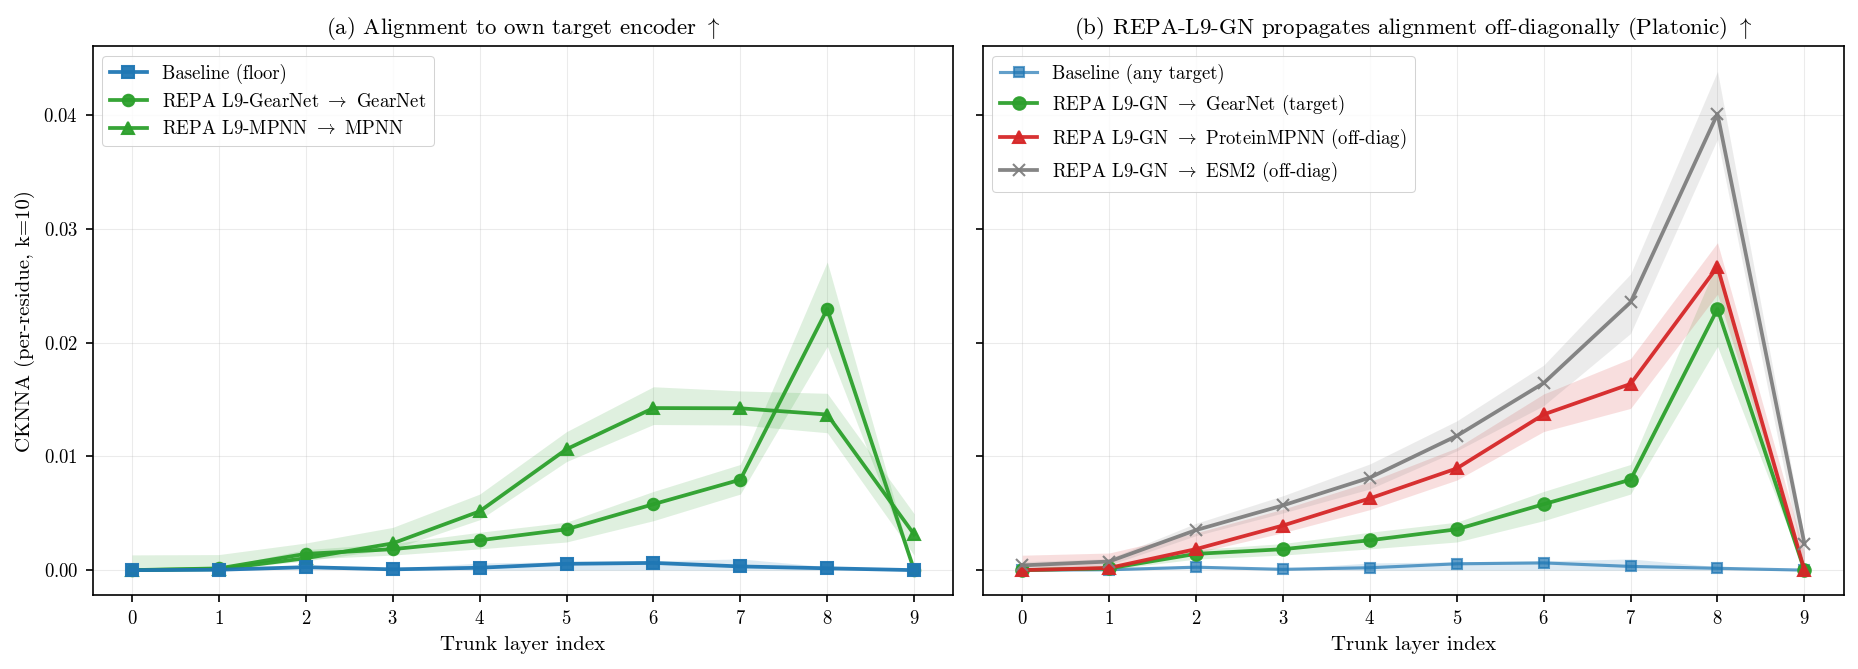
\includegraphics[width=\textwidth]{figures/fig03_alignment.png}
\caption{\textbf{REPA pulls the trunk's geometry toward the encoder's --- and toward encoders it was never trained on (Platonic convergence).} The baseline sits at the random floor at every layer (CKNNA $\approx 0$); REPA lifts per-residue alignment into a smooth profile that peaks one layer below the injection point and collapses at the velocity-output layer, cleanly separated from the baseline by the subsample bootstrap. Aligning to GearNet alone also pulls the trunk toward ProteinMPNN and ESM2 --- the off-diagonal Platonic signature, with ESM2 the strongest attractor. Absolute alignment is small (peak $\approx 0.02$--$0.05$ against $1$ for self-alignment), so we read direction and layer structure, not magnitude; the per-protein signal is far weaker and we do not claim a fold-level benefit. ($n{\le}256$ PDB, step 1M, $t{=}1.0$; per-residue CKNNA, $k{=}10$.)}
\label{fig:proteina-cknna}
\end{figure}
